\documentclass{article}
\usepackage{CJK}
\usepackage{indentfirst}
\usepackage{anysize}
\usepackage{graphicx}
\usepackage{subfigure}
\usepackage{array}
\usepackage{makecell}
\usepackage{url}
\usepackage{float}

%标题缩进
%\usepackage[bf, small]{titlesec}
%    \titleformat{\section}{\bf\large}{\thesection.\,}{0.24em}{}
%    \titlespacing{\section}{0cm}{*1.5}{*1.1}
%    \titleformat{\subsection}{\bf}{\thesubsection.\enspace}{0.5em}{}
%    \titlespacing{\subsection}{15pt}{*1.5}{*1.1}
%    \titleformat{\subsubsection}{}{\thesubsubsection.\,}{0.24em}{}
%    \titlespacing{\subsubsection}{30pt}{*1.5}{*1.1}

\linespread{1.5}


\marginsize{3.5cm}{3.5cm}{2cm}{2cm}
\setlength{\parindent}{2em}

\newcolumntype{L}[1]{>{\vspace{0.5em}\begin{minipage}{#1}\raggedright\let\newline\\
\arraybackslash\hspace{0pt}}m{#1}<{\end{minipage}\vspace{0.5em}}}
\newcolumntype{R}[1]{>{\vspace{0.5em}\begin{minipage}{#1}\raggedleft\let\newline\\
\arraybackslash\hspace{0pt}}m{#1}<{\end{minipage}\vspace{0.5em}}}
\newcolumntype{C}[1]{>{\vspace{0.5em}\begin{minipage}{#1}\centering\let\newline\\
\arraybackslash\hspace{0pt}}m{#1}<{\end{minipage}\vspace{0.5em}}}


%使得图片显示对应章节
\renewcommand\thefigure{\thesection.\arabic{figure}}
\makeatletter
\@addtoreset{figure}{section}
\makeatother

\begin{document} 
\begin{CJK}{UTF8}{gbsn}

\newcommand*{\titleGP}{\begingroup % Create the command for including the title page in the document
\centering % Center all text
\vspace*{\baselineskip} % White space at the top of the page

\rule{\textwidth}{1.6pt}\vspace*{-\baselineskip}\vspace*{2pt} % Thick horizontal line
\rule{\textwidth}{0.4pt}\\[\baselineskip] % Thin horizontal line

{\LARGE 基于多线程的电梯调度系统 \\ \vspace{2em} \begin{large} 操作系统课程设计 \end{large}}\\[0.2\baselineskip] % Title

\rule{\textwidth}{0.4pt}\vspace*{-\baselineskip}\vspace{3.2pt} % Thin horizontal line
\rule{\textwidth}{1.6pt}\\[\baselineskip] % Thick horizontal line

\scshape % Small caps
%利用操作系统中的多线程思想,自我实现电梯调度算法 \\[\baselineskip] % Tagline(s) or further description
operating system,  Spring 2017\par % Location and year

\vspace*{2\baselineskip} % Whitespace between location/year and editors

 By \\[\baselineskip]
{\Large1552674 李源 \par} % Editor list


\vfill % Whitespace between editor names and publisher logo

{\itshape Tongji University \\ School of Software Engineering \par}

\endgroup}


\titleGP % This command includes the title page
\clearpage
\tableofcontents
\clearpage

\section{项目背景}
\subsection{项目需求}
某一栋楼共有20层,五部互相关联的电梯,请基于线程的思想,模拟实现一个电梯调度的程序。程序中的功能包含以下部分:

(1)电梯内有楼层选择按钮、警报按钮;

(2)电梯外每一层有上行按钮、下行按钮;

(3)对于每一部电梯,有控制其工作、不工作的两个按钮;

(4)每一部电梯,能够显示所在楼层、运行状态、开关门状态。


\subsection{项目目的}

(1)通过控制电梯调度,实现操作系统调度过程;

(2)学习特定环境下多线程编程方法;

(3)学习调度算法。

\vspace{3em}

\section{需求分析}
根据实际情况,可将该电梯系统的需求分为两个部分。本文档首先对两个部分的需求进行分析,寻找、构建相应算法,并且考虑两者之间需求的冲突及其联系,最终构建出合理的项目方案。两个部分分别为:

(1)人在电梯内部,按下楼层,电梯将人送到指定楼层,即内部请求;

(2)人在电梯外某一层,按下向上或向下按钮,选择一部电梯来接人,即外部请求。

\subsection{电梯内部请求}
针对项目需求和项目目的,可以将电梯内部需求,分为如下几个方面:

(1)当人处在电梯内部时,可以按下楼层选择按钮,到达其想去的楼层。可供选择的楼层为1-20层,共20层;

(2)电梯当前所处的楼层能够清晰地显示;

(3)当电梯达到某一楼层时,会开门和关门;

(4)电梯可以处于运行和不运行两个状态;

(5)电梯处于运行状态,可同时接收内部请求和外部请求;电梯处于不运行状态,电梯会停在当前楼层,且不接收任何请求;

(6)五个电梯运行互不相干扰。

结合这6点,可设计电梯内部应该有20个电梯选择按钮、2个控制电梯运行按钮;以及显示楼层、显示开关门、显示电梯运行状态这3个小界面。在之后的项目实现部分,将对如上需求提出具体的实现策略。

\subsection{电梯外部请求}
针对项目需求和项目目的,可以将电梯外部需求,分为如下几个方面:

(1)对于每一层,能够请求向上和向下;

(2)当请求发出后,调度系统会立即选择一个电梯,将该请求加入该电梯的响应队列。并且在之后完成该请求;

(3)除非接收请求的电梯出现故障,否则请求将肯定被实现;

(4)电梯外部请求和内部请求对于某一个电梯可以同时响应。

结合这4点,可设计电梯外部每一层均有一个上行按钮和下行按钮,共$20*2$个;且按钮应该和楼层一一对应。

\subsection{两部分冲突及联系}

综上,我们得到了电梯系统的两部分的需求。对于两部分之间的冲突,主要有如下两个方面:

(1)对于某一部电梯,能够同时接收内部、外部请求;

(2)对于某一部电梯,其接收到的内部、外部请求都能够实现,且按照一定的顺序;

结合这2点,可考虑在设计电梯调度算法时,可以设置两个独立函数分别接收内部、外部请求;在电梯接收到请求后,将两种请求视为同一请求,完成对其的实现。

\vspace{3em}

\section{调度算法}

根据前文对本电梯系统的分析,以及对两种请求的具体考虑,可以将该调度算法细分为两个部分:

(1)电梯响应请求,对于外部请求,需选择适合的电梯响应该请求;

(2)电梯对接收到的请求完成实现,即前往对应楼层。

具体算法的思路和实现如下。

\subsection{响应请求算法}

每部电梯含有一个数组,用于存放楼层是否发出请求。

对于内部请求,当某一层按下,即发出请求后,直接将该请求放入数组当中。

\clearpage

对于外部请求,当某一层按下,选择一个合适的电梯响应该请求,其步骤如下:

(1)系统首先考虑将请求分配给离该层最近的、处于闲置的电梯;

(2)如果所有电梯均处在运动或不运行状态,则考虑分配给正在靠近该层、且最近的电梯;

(3)如果前面两点均没有电梯满足,则按照轮转的思想,将请求分配给一个正在运行的电梯;

(4)如果所有电梯均处于不运行状态,则该请求作废。

\subsection{实现请求算法}

首先,为了简化考虑,当电梯接收到一个请求并且响应时,会将外部、内部请求均视为同一类型的请求,即都要求电梯前往某一楼层。那么,电梯可按如下步骤实现该请求:

(1)当电梯处于闲置状态时,会监测是否收到请求;

(2)一旦收到,电梯会根据请求从更高(或更低)楼层传来,转换为上行(或下行);

(3)当电梯开始上行(或下行)后,每到一层,检测该楼层是否有内部或外部请求。如果有,则执行;

(4)同时,电梯到达一层后,会监测其上方(或下方)是否还有请求。如果有,电梯继续上行一层;如果没有,则转化为闲置状态。


\subsection{调度算法示意图}


\begin{figure}[!h]
\centering
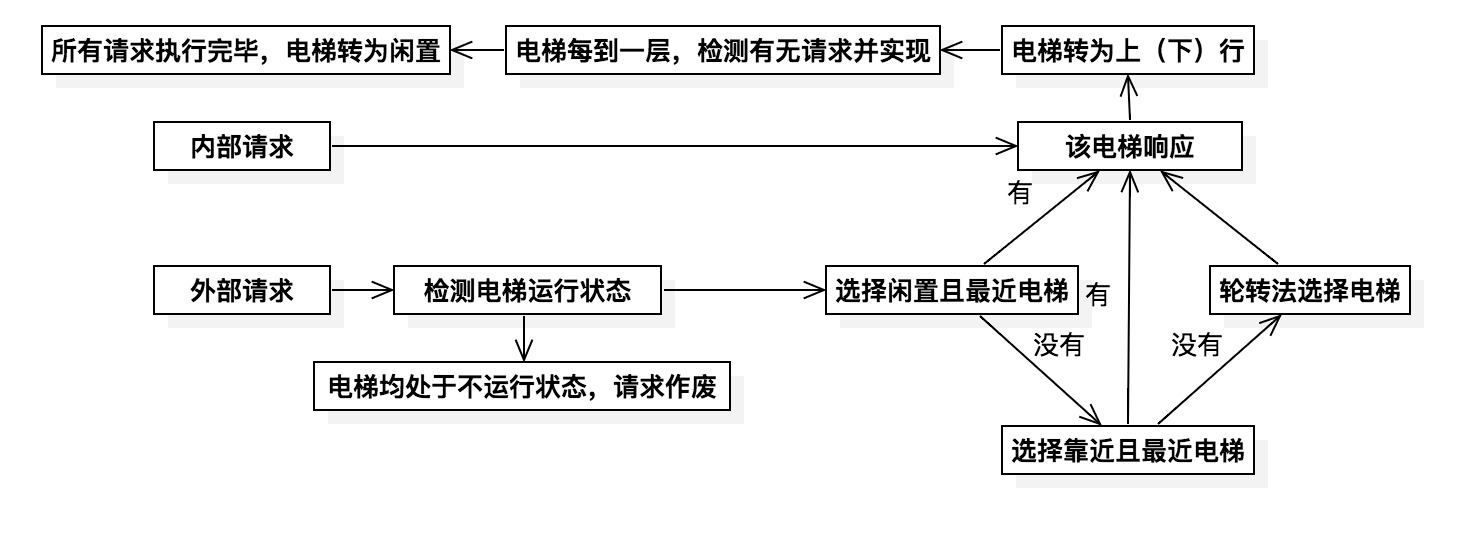
\includegraphics[width=1.1\textwidth]{1.jpg}
\caption{调度算法示意图}
\end{figure}


\clearpage

\section{系统实现}
根据需求分析,可以设计电梯系统的界面如下:
\begin{figure}[!h]
\centering
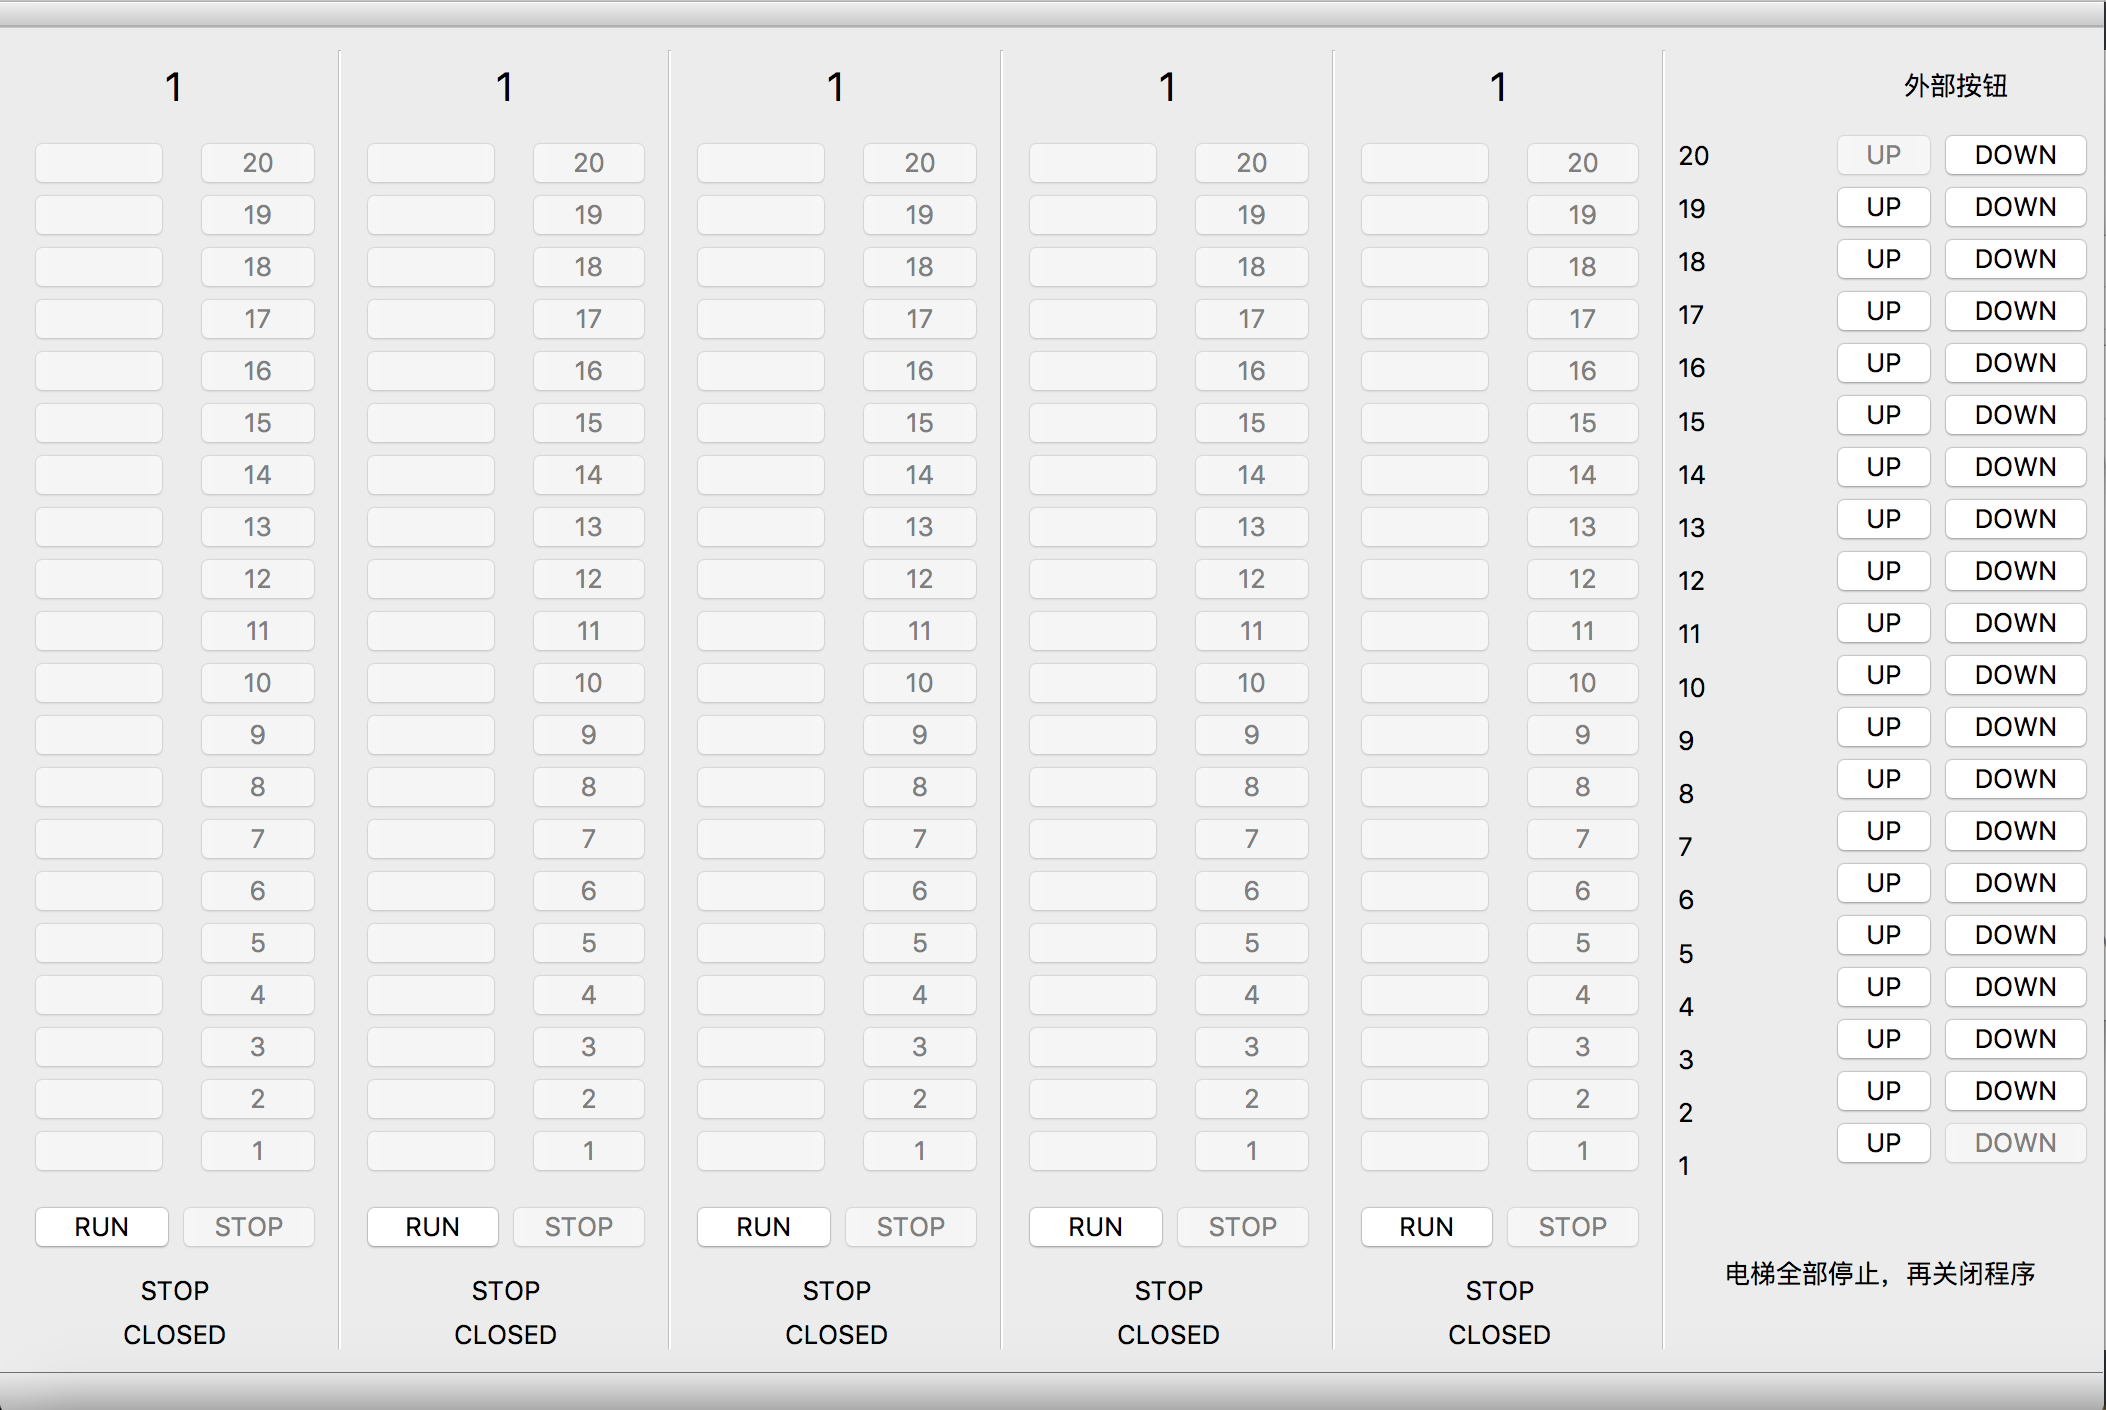
\includegraphics[width=0.77\textwidth]{2.png}
\caption{系统界面图}
\end{figure}

该界面可分为6个部分,左边5个部分对应5个电梯,最右边为外部请求按钮。

\subsection{电梯界面}
电梯界面各部分表达的内容如下:
\begin{figure}[!h]
\centering
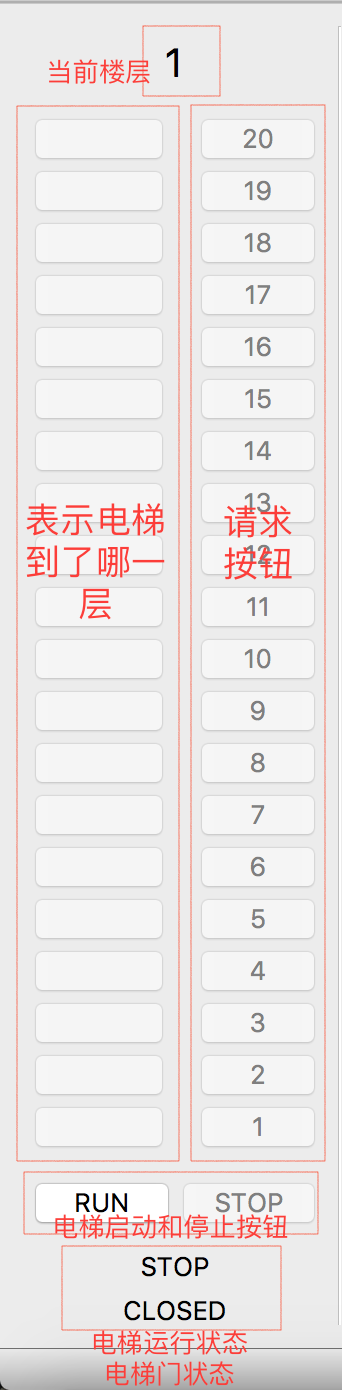
\includegraphics[width=0.14\textwidth]{3.png}
\caption{电梯界面图}
\end{figure}

\clearpage
每一部电梯在初始时均为不运行,即“STOP”状态。按下“RUN”按钮后,电梯启动,且左侧显示电梯当前所在楼层:

 \begin{figure}[H]  
 \centering
  \subfigure[电梯不运行状态]{
    \label{fig:subfig:a} %% label for first subfigure
    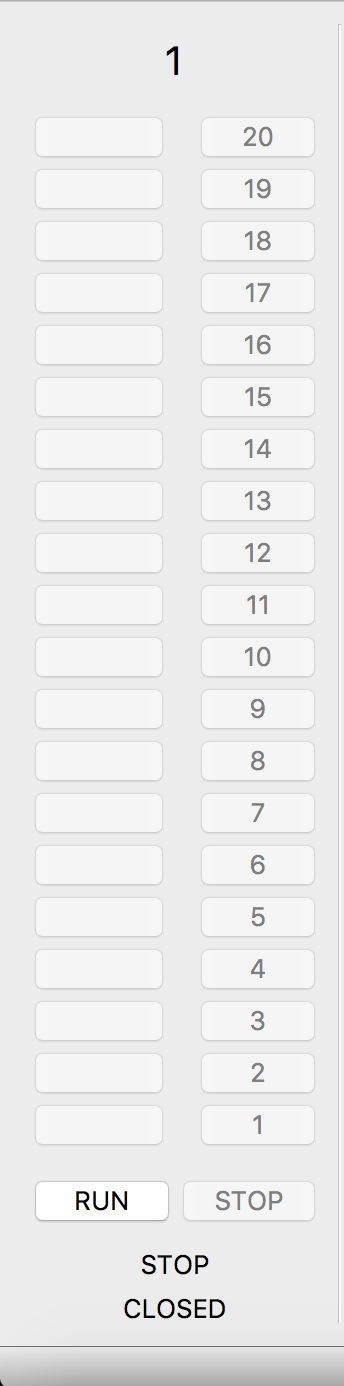
\includegraphics[width=0.13\textwidth]{4.PNG}}
  \hspace{0.5in}
  \subfigure[电梯运行状态]{
    \label{fig:subfig:b} %% label for second subfigure
    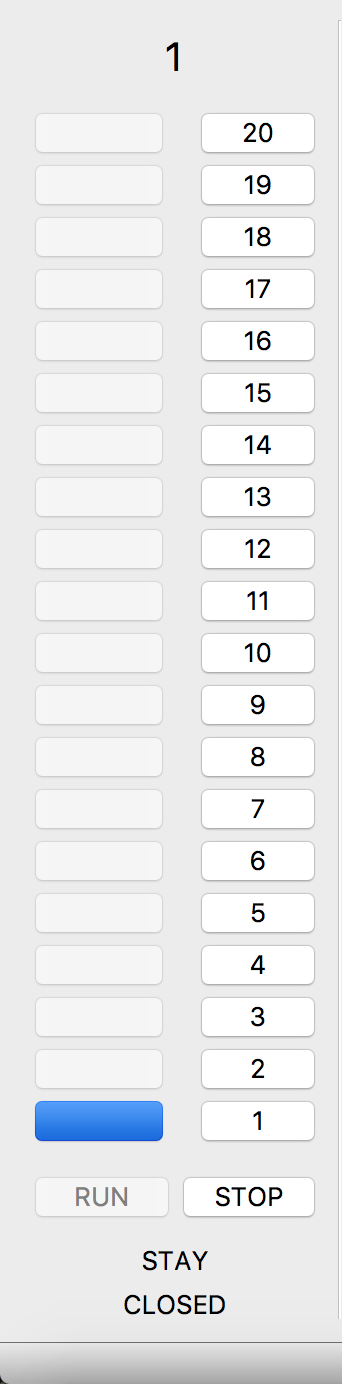
\includegraphics[width=0.13\textwidth]{5.PNG}}
   
  \caption{电梯状态示意图}
  \label{fig:subfig} %% label for entire figure
 \end{figure}

当电梯启动,处于运行状态后,即可正常响应、实现请求,如下图:

\begin{figure}[!h]
\centering
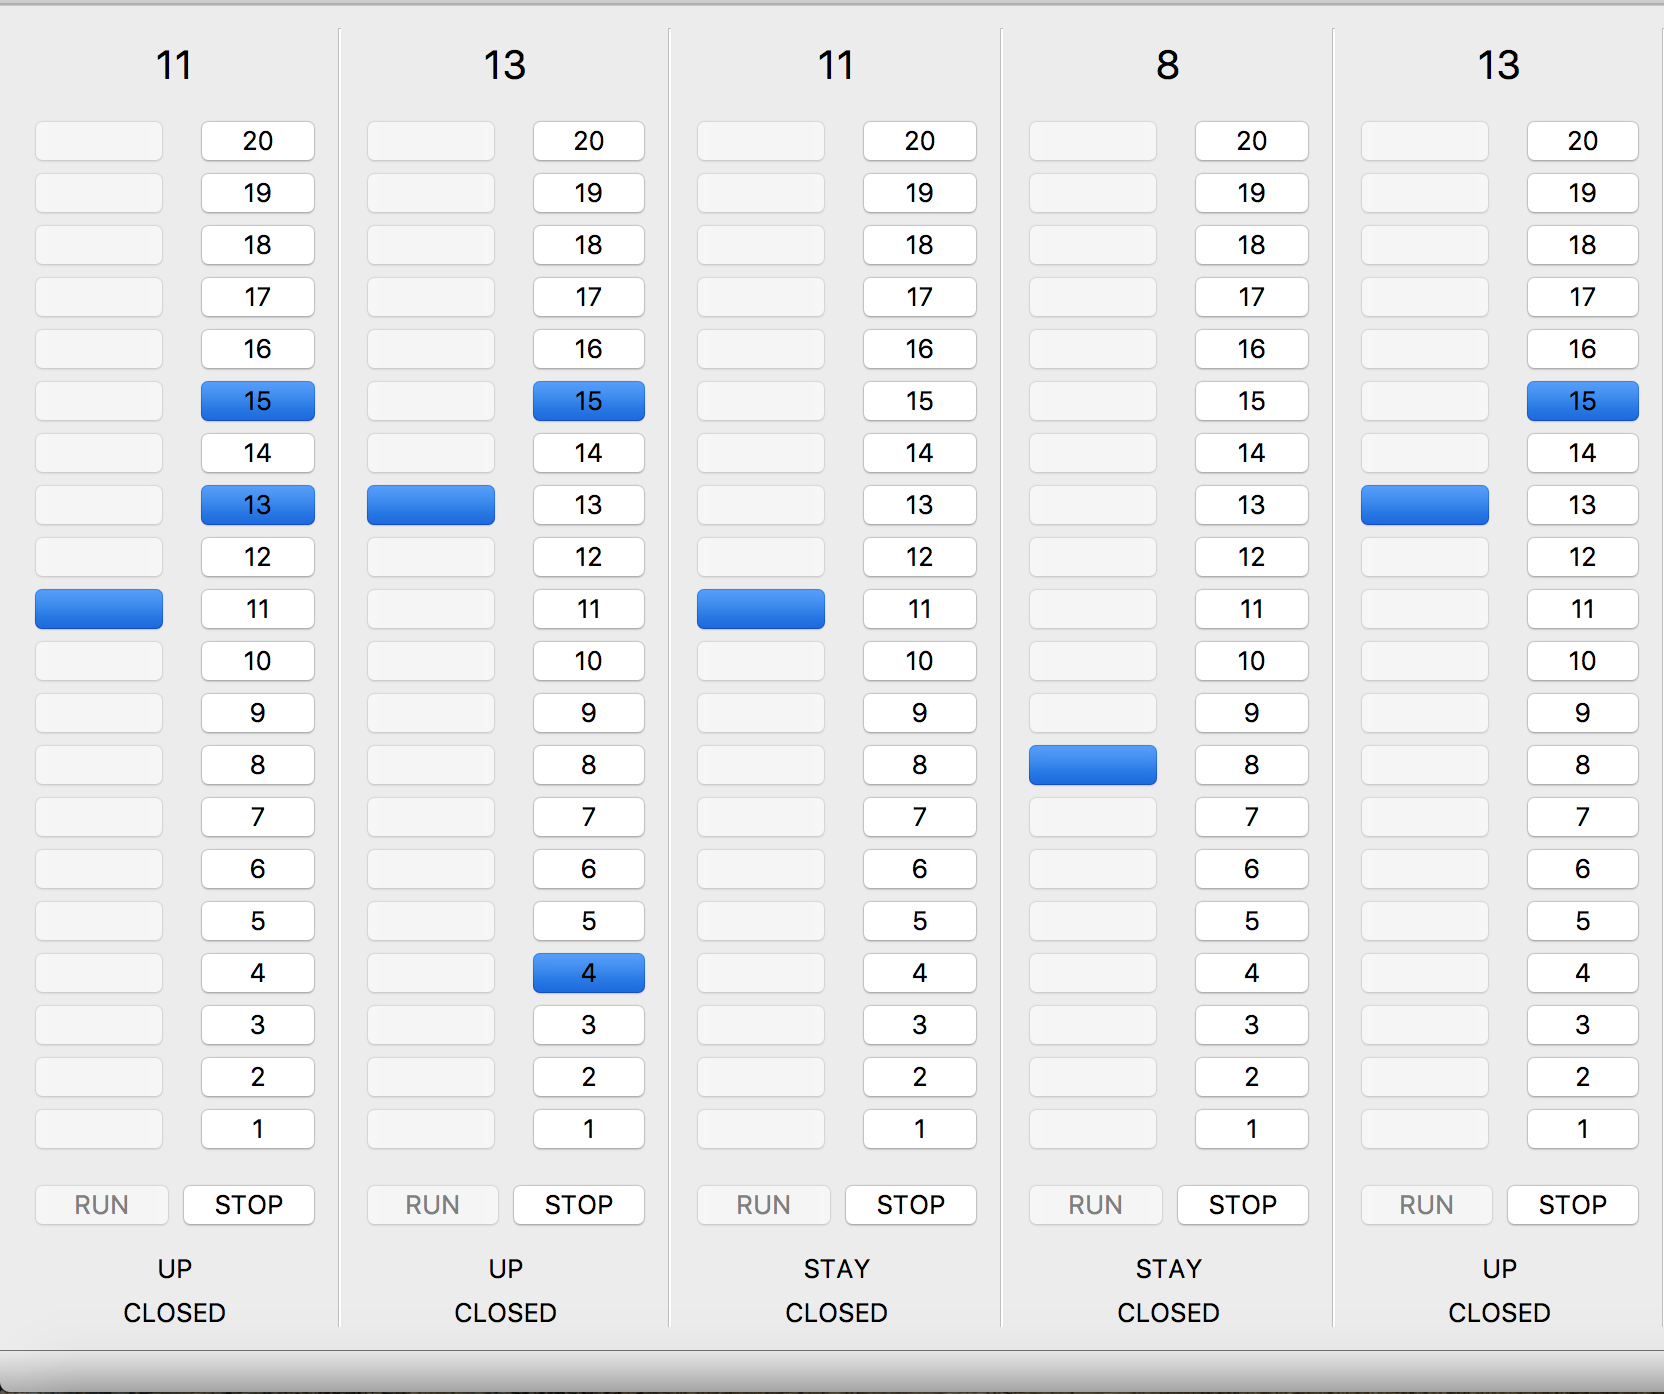
\includegraphics[width=0.78\textwidth]{6.png}
\caption{电梯运行界面}
\end{figure}

\subsection{外部按钮界面}
界面最右边为外部请求按钮界面,各部分表达的内容如下:
\begin{figure}[!h]
\centering
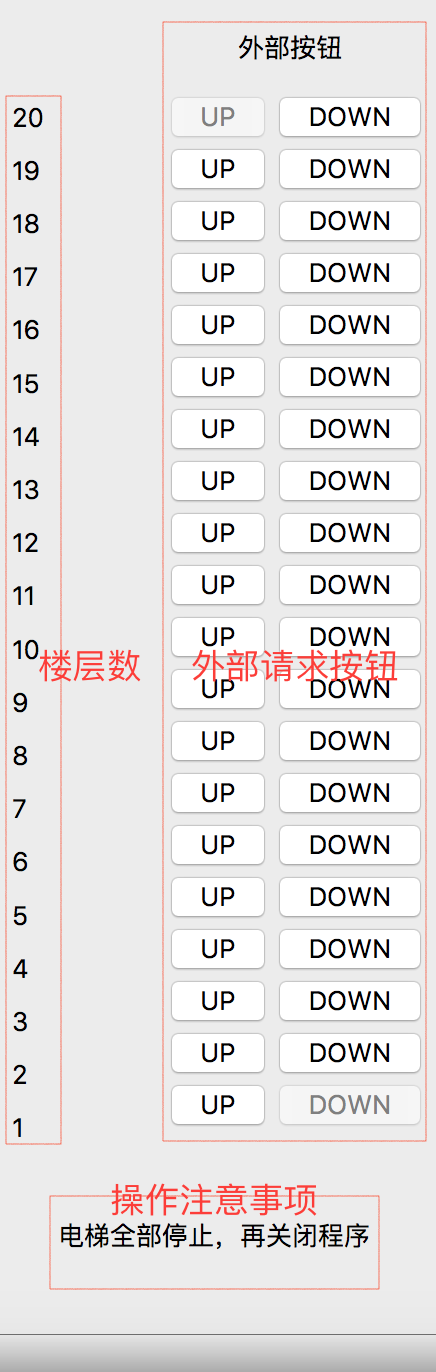
\includegraphics[width=0.15\textwidth]{7.png}
\caption{外部按钮界面图}
\end{figure}

当有电梯处于运行状态时,即可响应外部按钮发送的请求,如下图:
\begin{figure}[!h]
\centering
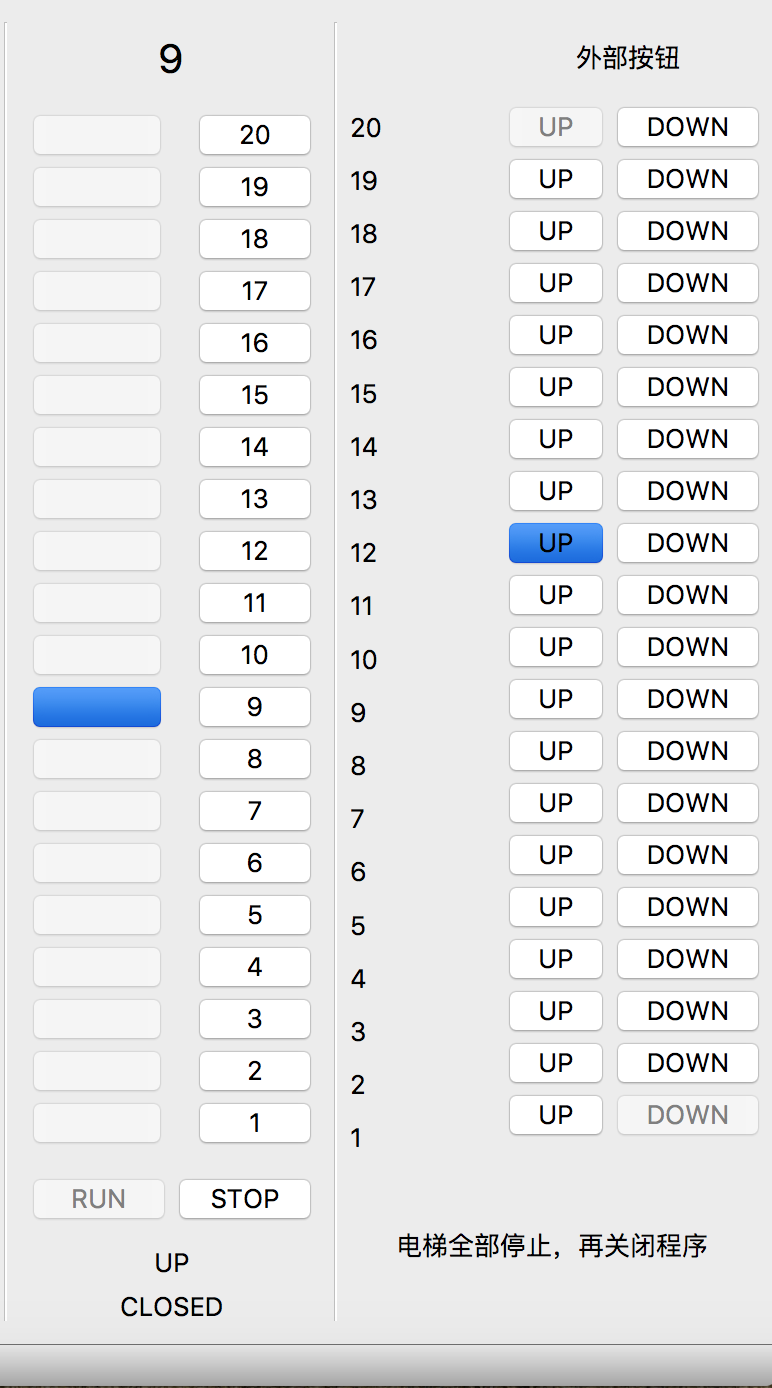
\includegraphics[width=0.25\textwidth]{8.png}
\caption{电梯响应外部请求}
\end{figure}

\subsection{演示视频}
具体运行效果,可见提交文件中的演示视频。

\subsection{注意事项}
(1)当电梯在运行过程按下“STOP”按钮,会使该电梯接收到的所有请求作废,电梯停于当前楼层,且不再响应请求。

(2)应确保所有电梯都处于不运行,即“STOP”状态,再关闭程序,否则可能出现异常关闭。

\vspace{3em}
\section{开发环境}
\begin{itemize}
	\item 系统:macOS Sierra (version 10.12.4)
	\item IDE:Qt Creator 4.2.1, Based on Qt 5.8.0 (Clang 7.0 (Apple), 64 bit)
	\item 语言: C++
\end{itemize}

\vspace{3em}
\section{提交内容}
\begin{itemize}
	\item 源代码
	\item assignment1.app 可执行文件(需在mac系统下使用)
	\item assignment1.dmg 安装包(需在mac系统下使用)
	\item 说明文档
	\item 演示视频
\end{itemize}

\end{CJK}
\end{document}